\documentclass[11pt]{article}

\usepackage[a4paper,margin=1in]{geometry}
\usepackage{amsmath,amssymb}
\usepackage{booktabs}
\usepackage{longtable}
\usepackage{array}
\usepackage{graphicx}
\usepackage{hyperref}
\usepackage{xcolor}
\usepackage{tikz}
\usepackage{listings}

\hypersetup{
  colorlinks=true,
  linkcolor=blue!55!black,
  urlcolor=blue!55!black,
  citecolor=blue!55!black
}

\lstdefinestyle{trap}{
  basicstyle=\ttfamily\small,
  breaklines=true,
  columns=fullflexible,
  frame=single,
  framerule=0.2pt,
  rulecolor=\color{black!25}
}
\lstset{style=trap}

\DeclareRobustCommand{\code}[1]{\texttt{\detokenize{#1}}}
\newcommand{\R}{\mathbb{R}}
\newcommand{\DC}{\overline{DC}}
\newcommand{\Area}{\operatorname{Area}}

\title{Interval Verification Documentation for \code{TrapeziumFence}}
\author{}
\date{September 2026}

\begin{document}
\maketitle

\begin{abstract}
This document describes the architecture, verification logic, functions, and
recorded experiments for the \code{TrapeziumFence} package.  The package verifies
upper bounds for the normalized shortest equal-area fence in convex
quadrilaterals and also records exclusions from the conditional equality class
of Proposition~17.
The search subdivides a four-dimensional rectangle of coordinates for the two
free vertices \(A,B\).  Each leaf rectangle is either discarded as certainly
inadmissible, certified as having a shortest fence value below a threshold
\(\theta\), proved incompatible with the opposite-pair equality hypothesis, or
retained as an unresolved survivor.  The certificate verifier re-checks both
the metadata, local leaf claims, and global dyadic tiling of the original
domain.
\end{abstract}

\tableofcontents

\section{Mathematical Normalization}

The package studies convex quadrilaterals \(DCBA\) with \(D=(0,0)\),
\(C=(1,0)\), \(B=(b_1,b_2)\), and \(A=(a_1,a_2)\).  The side \(DC\) is assumed
to be a longest side and is normalized to length \(1\).  This loses no
generality for the target functional, because fence lengths are divided by
\(\sqrt{\Area(DCBA)}\).  A quadrilateral with a longer side can be rescaled and
appears in another copy of the normalized search.

The raw search box is
\[
  b_1\in[0,2],\qquad b_2\in[0,1],\qquad
  a_1\in[-1,1],\qquad a_2\in[0,1].
\]
The admissibility predicate keeps only boxes that may contain counterclockwise
convex quadrilaterals whose non-base side lengths are at most \(1\):
\[
  |CB|\le 1,\qquad |BA|\le 1,\qquad |AD|\le 1.
\]

The C implementation and JSONL records still use the legacy coordinate slots
\((c_1,c_2,d_1,d_2)\).  In the public notation of this document these slots
mean \((b_1,b_2,a_1,a_2)\).

For a quadrilateral \(Q=DCBA\), the code computes six scale-invariant
fence-construction candidate values \(F_i(Q)\).  Proposition~6 gives the exact
representation
\[
  \Phi(Q) = \min_{0\le i<6} F_i(Q).
\]
In particular, each candidate is an upper bound for \(\Phi(Q)\).
The six items are four vertex-angle candidates and two exact opposite-edge-pair
candidates.  A box is certified below \(\theta\) when at least one finite
candidate enclosure has upper endpoint at most \(\theta\).  Equivalently, the
code takes the smallest finite candidate upper endpoint; this is a rigorous
one-sided upper bound for \(\min_i F_i\), even if another candidate failed to
produce a finite enclosure on a coarse box.
Consequently, certified boxes are one-sided exclusions for the problem
\(\Phi(Q)>\theta\): they prove that no admissible quadrilateral in the box has
normalized shortest fence value above the threshold.

\section{Package Architecture}

The C implementation is arranged in layers:

\begin{description}
  \item[\code{geom.c}, \code{geom.h}] Arb arithmetic wrappers, four-variable
  forward-mode automatic differentiation jets, and basic point/vector
  operations.

  \item[\code{series.c}, \code{series.h}] Rigorous enclosures for
  \(g(\gamma)=\gamma/\sin\gamma\) and \(g'(\gamma)\), used by the
  parallel-safe opposite-pair formula when the supporting lines are nearly
  parallel (that is, near \(\gamma=0\) or \(\gamma=\pi\)).

  \item[\code{functionals.c}, \code{functionals.h}] Construction of the six
  explicit fence-construction candidates, natural and centered interval
  enclosures, the one-sided minimum bound used by certification, and the optional
  \nolinkurl{functionals_opposite_pairs_disjoint} pair-compatibility test.
  Items 4 and 5 use the geometric sectors containing the quadrilateral and are
  exact opposite-pair construction values, not arbitrary majorants; the
  compatibility test relies on this contract.

  \item[\code{admissible.c}, \code{admissible.h}] Conservative interval tests
  that discard boxes containing no admissible normalized quadrilateral, plus
  the flat/small-area certificate
  \nolinkurl{box_small_area_certifies_low}.

  \item[\code{threshold.c}, \code{threshold.h}] Exact decimal threshold parser
  and rational comparison helpers.  The literal passed to \code{--theta} is
  the mathematical constant used by certification; printed doubles are only
  diagnostic.

  \item[\code{search.c}, \code{search.h}] Dyadic subdivision engine.  It
  classifies boxes as discarded, certified low, flat-area low,
  pair-incompatible, or surviving; splits unresolved boxes; collects
  statistics; and can seed a refinement run from previous survivors.

  \item[\code{cert.c}, \code{cert.h}] JSONL certificate writer, stateless
  certificate verifier, and certificate assembler.  The verifier first checks
  the self-describing metadata line, then recomputes local claims and checks
  that all leaves tile the original domain by the same dyadic splitting rule.
  Missing dyadic children fail immediately.  The assembler replaces survivor
  leaves through a refinement chain.  It requires matching schema, exact
  threshold, enclosure form, half-domain choice, and root; the two auxiliary
  flags are combined by logical OR and the minimum component run precision is
  recorded in the assembled metadata.

  \item[\code{fence_validate.c}] Command-line front end for searching,
  refining, verifying, and evaluating a point.

  \item[\code{analyze_cert.py}] Safe postprocessing of certificate files.  It
  sums dyadic volumes and checks the strict admissible survivor core with exact
  rational endpoint arithmetic; it does not replace certificate verification.

  \item[\code{analyze_refinement_distances.py}] Distance-to-\(T^\ast\)
  postprocessor for the recorded refinement chain.  It reports
  ordinary floating-point distance diagnostics from each survivor rectangle
  to the displayed decimal reference trapezoid; these are not validated
  certificate bounds.

  \item[\code{tests/test_trap.c}] Unit tests for the reference trapezoid and
  strict threshold comparison, ordinary obtuse and near-\(\pi\) pair-bound
  formula agreement, value/derivative series evaluation, inadmissibility, one
  interior certification, the conditional pair-equality test, and the
  flat-area certificate.

  \item[\code{tests/test_cert_cli.sh}] CLI regression test for certificate
  verification, strict numeric parsing, legacy status compatibility, null
  diagnostic fields, dynamic-team termination, the debugging leaf cap, and
  fast failure on a missing certificate leaf.
\end{description}

\section{Rectangle Validation Logic}

\subsection{Cells}

A search cell is a four-dimensional rectangle
\[
  X =
  [b_{1}^{-},b_{1}^{+}]
  \times [b_{2}^{-},b_{2}^{+}]
  \times [a_{1}^{-},a_{1}^{+}]
  \times [a_{2}^{-},a_{2}^{+}].
\]
Equivalently, it is a product of two planar rectangles:
\[
  X_A=[a_{1}^{-},a_{1}^{+}]\times[a_{2}^{-},a_{2}^{+}],
  \qquad
  X_B=[b_{1}^{-},b_{1}^{+}]\times[b_{2}^{-},b_{2}^{+}].
\]
The initial cell has
\[
  X_A=[-1,1]\times[0,1],
  \qquad
  X_B=[0,2]\times[0,1].
\]

\begin{figure}[h]
\centering
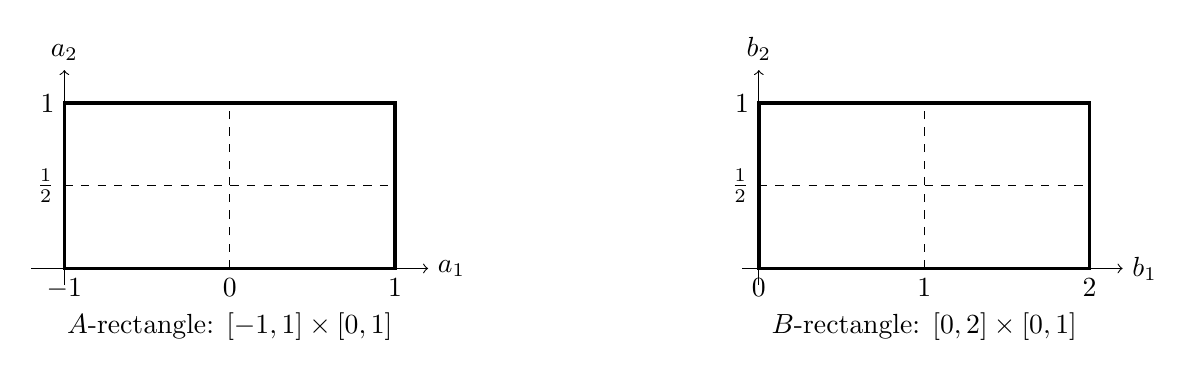
\begin{tikzpicture}[scale=2.1]
  \begin{scope}
    \draw[->] (-1.2,0) -- (1.2,0) node[right] {\(a_1\)};
    \draw[->] (-1,-0.1) -- (-1,1.2) node[above] {\(a_2\)};
    \draw[very thick] (-1,0) rectangle (1,1);
    \draw[dashed] (0,0) -- (0,1);
    \draw[dashed] (-1,0.5) -- (1,0.5);
    \node at (0,-0.35) {\(A\)-rectangle: \([-1,1]\times[0,1]\)};
    \node[below] at (-1,0) {\(-1\)};
    \node[below] at (0,0) {\(0\)};
    \node[below] at (1,0) {\(1\)};
    \node[left] at (-1,0.5) {\(\frac12\)};
    \node[left] at (-1,1) {\(1\)};
  \end{scope}
  \begin{scope}[xshift=3.2cm]
    \draw[->] (-0.1,0) -- (2.2,0) node[right] {\(b_1\)};
    \draw[->] (0,-0.1) -- (0,1.2) node[above] {\(b_2\)};
    \draw[very thick] (0,0) rectangle (2,1);
    \draw[dashed] (1,0) -- (1,1);
    \draw[dashed] (0,0.5) -- (2,0.5);
    \node at (1,-0.35) {\(B\)-rectangle: \([0,2]\times[0,1]\)};
    \node[below] at (0,0) {\(0\)};
    \node[below] at (1,0) {\(1\)};
    \node[below] at (2,0) {\(2\)};
    \node[left] at (0,0.5) {\(\frac12\)};
    \node[left] at (0,1) {\(1\)};
  \end{scope}
\end{tikzpicture}
\caption{Equal-axis initial planar grids for \(A\) and \(B\).  Combining one
rectangle from the \(A\)-grid with one rectangle from the \(B\)-grid gives a
four-dimensional cell.}
\end{figure}

\subsection{Splitting Rule}

The root spans are
\[
  (2,1,2,1)
\]
for the public coordinates \((b_1,b_2,a_1,a_2)\).  The search compares scaled widths
\[
  \frac{b_1^+-b_1^-}{2},\qquad
  b_2^+-b_2^-,\qquad
  \frac{a_1^+-a_1^-}{2},\qquad
  a_2^+-a_2^-.
\]
The coordinate with largest scaled width is bisected.  If the coordinate is
\(b_1\) or \(b_2\), only the \(B\)-rectangle changes; if it is \(a_1\) or
\(a_2\), only the \(A\)-rectangle changes.  This rule is deterministic and is
used by both the search and the certificate verifier.

\subsection{Leaf Classification}

For a box \(X\), the search applies the following logic:

\begin{enumerate}
  \item If \code{box\_certainly\_inadmissible} proves that the entire box
  violates convexity or side-length constraints, or lies wholly outside the
  optional selected symmetry half-domain, the leaf is written with status
  \code{discarded}.

  \item If \code{--flat-area-cert} is enabled and
  \code{box\_small\_area\_certifies\_low} proves the flat/small-area estimate
  below, the leaf is written with status \code{flat\_area}.  This is a genuine
  low-fence certificate.

  \item If \code{--pair-eq-cert} is enabled and
  \code{functionals\_opposite\_pairs\_disjoint} proves that the two
  opposite-pair fence intervals are disjoint, the leaf is written with status
  \code{pair\_incompatible}.  This proves that the leaf contains no
  quadrilateral satisfying the equality hypothesis of Proposition~17, but is
  not by itself a low-fence or global nonoptimality claim.

  \item Otherwise, \code{functionals\_min} takes the minimum of the upper
  endpoints of all finite candidate enclosures.  The resulting
  \(f_{\mathrm{hi}}\) is a rigorous one-sided upper bound for the six-item
  minimum.  If \(f_{\mathrm{hi}}\le\theta\), the leaf is written with status
  \code{certified}.  Its paired lower endpoint encloses the true minimum only
  when all six candidate enclosures are finite and is otherwise diagnostic.

  \item If the box is not certified and its largest scaled width is at most
  \code{wfloor}, it is written with status \code{survivor}.  A survivor is not
  evidence of optimality; it is merely an unresolved part of the outer
  neighborhood.

  \item Otherwise the box is split into two children and the process continues.
\end{enumerate}

The search can be restarted from survivors by passing \code{--refine FILE}.
Refinement outputs are partial certificates.  Use \code{--assemble} to replace
survivor leaves stage by stage and produce a complete certificate for the
original root box.

\subsection{Self-Describing Certificate Metadata}

Every JSONL certificate begins with a metadata line of schema version \(3\).
It records the threshold \(\theta\) as an exact decimal string, enclosure form,
half-domain flag, auxiliary-certificate flags, precision provenance, root box,
and splitter spans.  Leaf lines follow this first line.

The verifier reads \(\theta\), \code{form}, and \code{half} from the file.
Supplying \code{--theta}, \code{--form}, or \code{--half} during
\code{--verify} is only a cross-check: if a command-line value disagrees with
the certificate metadata, verification fails with \code{FAIL[meta]}.  This
prevents a certificate for one threshold from being silently audited as a
different, usually weaker, statement.

The exact \(\theta\) literal is parsed as a rational number.  Certified leaves
compare the Arb upper endpoint to this rational.  The flat-area certificate
compares the area upper endpoint to the exact rational \(\theta^2/4\), not to a
rounded floating-point value.  The metadata field \code{theta\_approx} and
printed decimal summaries are diagnostic only.

The assembler requires metadata in every input file.  Before replacing
survivor leaves, it checks equality of the schema, exact threshold, enclosure
form, half-domain choice, and root.  Auxiliary-certificate flags are combined
by logical OR and the assembled \code{run\_prec} is the minimum component
precision.  Old JSONL files without schema-3 metadata must be regenerated with
the current program before they can be audited or assembled.

\subsection{Certificate Semantics}

A complete verified certificate with \code{half=false} proves:
\[
  \text{every admissible quadrilateral outside the survivor union is either}
\]
\[
  \text{certified below \(\theta\) or incompatible with pair equality.}
\]
Statuses \code{certified} and \code{flat\_area} are low-fence certificates:
they prove \(\Phi(Q)\le\theta\) throughout the box.  Status
\code{pair\_incompatible} proves only that the two exact pair values cannot be
equal on the box.  Legacy schema-3 files spell this status \code{nonoptimal};
the verifier and postprocessors accept both strings.  The legacy name is not
an unconditional assertion that no optimizer can lie in the box.

Therefore a certificate with \code{--pair-eq-cert} enabled should be read as an
exclusion certificate conditional on Proposition~17.  The paper supplies its
equality hypothesis after reducing to analytic configurations in which both
opposite-pair fences are active; the equality is not claimed for every
optimizer.  The certificate does not prove that survivor boxes contain values
above \(\theta\), nor does it produce a lower bound for the true optimum.  It
gives an outer neighborhood for currently unresolved configurations in that
equality class.  With \code{half=true}, the displayed statement is restricted
to the selected representative half-domain; reflecting its survivor union
gives the corresponding full-domain outer neighborhood.

\section{Auxiliary Certificates}

\subsection{Opposite-Pair Equality}

The two opposite-pair candidates are exact fence-construction values.
They correspond to the pairs \((DC,BA)\) and \((CB,AD)\).
Proposition~17 assumes that these two
values agree; the analytic proof supplies this equality in the cases where
both pair fences are active.  The optional test \code{--pair-eq-cert} evaluates
interval enclosures for the two exact values.  If the finite intervals are
disjoint, no point in the box can satisfy the equality hypothesis, and the box
is written with status \code{pair\_incompatible}.

This test is independent of the threshold \(\theta\).  It removes regions from
the Proposition~17 equality class even when the current candidate-value
envelope is too wide to certify \(\Phi(Q)\le\theta\).  This use is sound only
because items 4 and 5 enclose exact pair-construction values, with the sector
containing the quadrilateral, rather than loose upper majorants.  It has no
standalone global-optimality meaning outside the analytic equality reduction.

\subsection{Flat and Small-Area Estimate}

Let
\[
  A_Q=\Area(DCBA),\qquad h=\max\{a_2,b_2\}.
\]
For the fence associated to the pair of opposite sides \((DC,BA)\), a direct
construction gives
\[
  L_{DC,BA}\le h.
\]
Indeed, the relevant separating curve can be chosen with length no larger than
the largest height of the two mobile vertices over the base line \(DC\).

For an admissible counterclockwise convex quadrilateral in the normalized
domain,
\[
  A_Q=\Area(DCB)+\Area(DBA)>\frac{b_2}{2},
  \qquad
  A_Q=\Area(DCA)+\Area(CBA)>\frac{a_2}{2}.
\]
Hence \(h\le 2A_Q\), and therefore
\[
  \frac{L_{DC,BA}}{\sqrt {A_Q}}\le \frac{h}{\sqrt {A_Q}}\le 2\sqrt {A_Q}.
\]
Consequently, if interval arithmetic proves
\[
  A_{\mathrm{ub}}\le \frac{\theta^2}{4},
\]
then the whole box has normalized shortest fence value at most \(\theta\).
This is implemented by \code{box\_small\_area\_certifies\_low} and recorded
with status \code{flat\_area}.

For the threshold used below,
\[
  \theta=1.0496,\qquad
  \theta^2=1.10166016,\qquad
  \frac{\theta^2}{4}=0.27541504.
\]

\subsection{Angle Consequence}

The vertex fence at an angle \(\alpha\) has normalized upper bound
\(\sqrt{\alpha}\).  Thus, if the smallest angle of \(DCBA\) is less than
\(\theta^2\), the quadrilateral is already below threshold.  Any possible
above-threshold optimizer must therefore have all four angles at least
\(\theta^2\), so its largest angle is at most
\[
  2\pi-3\theta^2.
\]
For \(\theta=1.0496\), ordinary high-precision evaluation gives the
diagnostic approximation
\[
  2\pi-3\theta^2 \approx 2.9782048271795865\text{ radians}
  \approx170.63856712287902^\circ,
\]
if \(\alpha_{\max}\) is the largest angle, its guaranteed gap from a straight
angle satisfies
\[
  \pi-\alpha_{\max}\ge 3\theta^2-\pi
  \approx0.16338782641020676\text{ radians}.
\]
The exact symbolic expressions, rather than these rounded diagnostics, carry
the preceding inequality directions.
This angle observation explains why very flat quadrilaterals should not be
optimal.  The implemented small-area certificate above is the direct
quantitative exclusion used in the current computation.

\section{Functional Bounds}

\subsection{Vertex Bounds}

For a vertex \(V\) with neighboring vertices \(P,Q\), the vertex item is
\[
  F_V = \sqrt{\angle PVQ}.
\]
The angle is computed as
\[
  \operatorname{atan2}\bigl(|(P-V)\times(Q-V)|,\ (P-V)\cdot(Q-V)\bigr).
\]
If a coarse interval contains a degenerate vertex case where \code{atan2}
becomes indeterminate, the value interval is clamped conservatively to
\([0,\pi]\), and derivative information is treated as indeterminate.  In
centered mode this forces a conservative fallback to the natural enclosure.

\subsection{Opposite-Pair Candidates}

There are two exact opposite-pair candidate values: \((DC,BA)\) and
\((CB,AD)\).  Give the two sides their counterclockwise boundary directions
\(d_1,d_2\).  The aperture of the sector cut out by their inward half-planes,
and hence the sector containing the quadrilateral, is
\[
  \gamma=\operatorname{atan2}(|d_1\mathbin\times d_2|,-d_1\mathbin\cdot d_2)
  \in[0,\pi].
\]
It may be obtuse; it is not always the acute angle between the unoriented
supporting lines.  Let \(A_Q=\Area(DCBA)\).  The implementation uses two
algebraically identical formulas.

The branch decision uses the acute separation
\(\delta=\operatorname{atan2}(|d_1\times d_2|,|d_1\cdot d_2|)\).  Away from
parallelism the apex form is used.  Let \(O\) be the intersection point of the
two supporting lines, and let \(T_0,T_1\) be the areas of the two triangles
formed by the non-pair edges and \(O\).  Then
\[
  F_{\mathrm{pair}}^2 = \frac{\gamma(T_0+T_1)}{A_Q}.
\]
Near parallelism, the symmetric formula is used:
\[
  F_{\mathrm{pair}}^2 =
  \frac{\gamma}{\sin\gamma}\,
  \frac{p_a+p_b}{2A_Q},
\]
where each \(p\) is a product of distances from the endpoints of one non-pair
edge to the two opposite supporting lines.  This form avoids the unstable
intersection point \(O\) when the acute separation
\(\delta=\min\{\gamma,\pi-\gamma\}\) is small.

\subsection{Natural and Centered Enclosures}

The natural enclosure evaluates each expression directly over interval boxes.
The centered enclosure uses a mean-value form
\[
  F_i(m) + \sum_{k=0}^{3} \partial_k F_i(X)\,[-r_k,r_k],
\]
where \(m\) is the coordinate midpoint and \(r_k\) is half the coordinate
width.  The derivatives \(\partial_kF_i(X)\) are obtained by forward-mode
automatic differentiation over Arb balls.  In centered mode the code combines
the centered and natural enclosures conservatively: if both are finite and
overlap, their intersection is used; if they are finite but disjoint, their
hull is used; if one is non-finite, the finite one is used.

\section{Function Reference}

This section lists the public routines and selected static helpers by module.
Static helpers are included when they encode important proof logic.

\subsection{\code{geom.c}/\code{geom.h}}

\begin{longtable}{>{\ttfamily}p{0.30\textwidth}p{0.62\textwidth}}
\toprule
Function & Purpose \\
\midrule
\endhead
jet\_init & Initializes the value ball and all four derivative balls of a jet. \\
jet\_clear & Clears all Arb storage owned by a jet. \\
jet\_set & Copies a jet value and its derivative enclosures. \\
jet\_set\_var & Seeds one moduli coordinate as an automatic-differentiation variable with derivative \(1\) in coordinate \(k\). \\
jet\_set\_const & Sets a constant Arb value and zero derivatives. \\
jet\_set\_si & Sets a signed integer constant and zero derivatives. \\
jet\_add & Adds two jets componentwise. \\
jet\_sub & Subtracts two jets componentwise. \\
jet\_neg & Negates value and derivatives. \\
jet\_mul & Multiplies jets using the product rule; temporaries allow aliasing. \\
jet\_div & Divides jets using the quotient rule; non-finite balls are preserved when the denominator straddles zero. \\
jet\_sqr & Squares a jet and applies \(d(a^2)=2a\,da\). \\
jet\_sqrt & Applies square root with derivative \(da/(2\sqrt a)\).  Degenerate input may produce non-finite derivative enclosures, which higher layers handle conservatively. \\
jet\_abs & Computes \(|a|\).  If the value straddles zero, the value becomes \([0,\sup |a|]\) and derivatives receive sign uncertainty. \\
jet\_atan2 & Computes \(\operatorname{atan2}(y,x)\) and its derivative \((x\,dy-y\,dx)/(x^2+y^2)\). \\
jet\_mul\_si & Multiplies a jet by a signed integer. \\
jet\_mul\_arb & Multiplies a jet by a scalar Arb constant. \\
jpt\_init & Initializes a two-coordinate jet point. \\
jpt\_clear & Clears a jet point. \\
jpt\_sub & Subtracts two jet points. \\
jet\_cross & Computes the two-dimensional cross product of two jet vectors. \\
jet\_dot & Computes the dot product of two jet vectors. \\
trap\_cross & Scalar Arb cross product for raw vector components. \\
trap\_dot & Scalar Arb dot product for raw vector components. \\
\bottomrule
\end{longtable}

\subsection{\code{series.c}/\code{series.h}}

\begin{longtable}{>{\ttfamily}p{0.30\textwidth}p{0.62\textwidth}}
\toprule
Function & Purpose \\
\midrule
\endhead
series\_build & Static initializer that computes Taylor coefficients for \(\gamma/\sin\gamma\) as rational numbers and stores them as high-precision Arb balls. \\
ensure\_coeffs & Static guard that lazily initializes the coefficient table; protected by an OpenMP critical section when OpenMP is enabled. \\
series\_cleanup & Clears cached coefficient balls.  Called by the CLI and tests before exit. \\
ghi\_ball & Static helper that turns the upper endpoint of a \(\gamma\) interval into a thin Arb ball. \\
nonnegative\_below\_pi & Static helper that intersects the geometric angle with \([0,\infty)\) and fails closed unless its upper endpoint is proved strictly below \(\pi\). \\
nonnegative\_half\_pi & Static helper that additionally verifies the Taylor-series domain \([0,\pi/2]\). \\
gamma\_over\_sin\_series & Taylor-series enclosure for \(g(\gamma)=\gamma/\sin\gamma\), with a rigorous positive tail bound. \\
gamma\_over\_sin\_value & Monotone endpoint enclosure for \(g(\gamma)\), avoiding the removable \(0/0\) singularity. \\
gamma\_over\_sin\_deriv & Encloses \(g'(\gamma)\) by direct formula away from zero and by series near zero. \\
jet\_gamma\_over\_sin & Applies \(g\) to a jet using the value enclosure and derivative enclosure. \\
\bottomrule
\end{longtable}

\subsection{\code{functionals.c}/\code{functionals.h}}

\begin{longtable}{>{\ttfamily}p{0.30\textwidth}p{0.62\textwidth}}
\toprule
Function & Purpose \\
\midrule
\endhead
vbound & Static helper for the vertex bound \(\sqrt{\angle PVQ}\). \\
pdist & Static helper for the distance from a point to a line, used in the parallel-safe pair formula. \\
tri\_area & Static helper for triangle area \( \frac12 |(Q-P)\times(O-P)| \). \\
pair\_bound & Static helper implementing the exact opposite-pair candidate value for the sector containing the quadrilateral.  It selects the apex formula or the parallel-safe formula using the acute separation of the supporting lines unless a test forces one; both formulas represent the same construction. \\
compute\_items & Static builder for the six candidate-value jets from the four coordinate jets.  In public notation it constructs \(A_Q=(b_2+b_1a_2-a_1b_2)/2\); in the legacy implementation slots this is \((c_2+c_1d_2-d_1c_2)/2\). \\
functionals\_eval & Public routine that encloses all six candidate values on a coordinate box, in natural or centered form. \\
functionals\_pair\_forced & Test hook that evaluates one pair candidate at a point while forcing the apex or parallel-safe formula. \\
functionals\_min & Takes the minimum of the finite candidate upper endpoints, giving the one-sided bound needed for certification.  Its lower endpoint is a full minimum bound only when all six items are finite.  If all six are non-finite, the result is \(+\infty\), so the search cannot certify the box. \\
functionals\_\allowbreak opposite\_\allowbreak pairs\_\allowbreak disjoint & Encloses the two exact opposite-pair candidate values and returns true only when both finite intervals are disjoint, certifying incompatibility with the equality hypothesis of Proposition~17. \\
\bottomrule
\end{longtable}

\subsection{\code{admissible.c}/\code{admissible.h}}

\begin{longtable}{>{\ttfamily}p{0.30\textwidth}p{0.62\textwidth}}
\toprule
Function & Purpose \\
\midrule
\endhead
set\_box & Static helper converting double endpoints into an Arb interval. \\
sqlen & Static helper computing squared vector length in Arb arithmetic. \\
box\_\allowbreak certainly\_\allowbreak inadmissible & Returns true when a whole box is proved inadmissible, or in half-domain mode when it lies wholly outside the selected representative half.  It checks CCW convexity through cross products, side lengths through squared distances, and optionally the reflection condition \(a_1+b_1\ge1\) (stored internally as \(c_1+d_1\ge1\)). \\
box\_\allowbreak small\_\allowbreak area\_\allowbreak certifies\_\allowbreak low & Returns true only when the interval upper bound for area satisfies \(A_{\rm ub}\le\theta^2/4\), so the estimate \(L_{DC,BA}/\sqrt {A_Q}\le 2\sqrt {A_Q}\) proves the box below threshold. \\
\bottomrule
\end{longtable}

\subsection{\code{search.c}/\code{search.h}}

\begin{longtable}{>{\ttfamily}p{0.30\textwidth}p{0.62\textwidth}}
\toprule
Function & Purpose \\
\midrule
\endhead
search\_root\_box & Writes the full coordinate domain \([0,2]\times[0,1]\times[-1,1]\times[0,1]\). \\
st\_init & Static stack initializer for pending boxes. \\
st\_free & Static stack destructor. \\
st\_push & Static stack push with geometric reallocation. \\
st\_pop & Static stack pop; returns false when empty. \\
widest\_coord & Static helper selecting the coordinate with largest root-span-scaled width. \\
classify & Static core classifier.  It applies inadmissibility, optional flat-area certification, optional pair-equality incompatibility, functional certification, optional adaptive precision, survivor flooring, and child generation. \\
stats\_add\_leaf & Static statistics accumulator for a final leaf. \\
run\_serial & Static depth-first serial driver over a seeded stack. \\
run\_parallel & Static OpenMP driver using a shared stack, critical sections for stack/statistics updates, atomic termination state, and the actual runtime team size for dynamic teams. \\
run\_stack & Static dispatcher that initializes statistics and selects serial or parallel execution. \\
search\_run & Starts a search from the root box. \\
search\_run\_seeded & Starts a search from explicit seed boxes, used by \code{--refine}. \\
\bottomrule
\end{longtable}

\subsection{\code{threshold.c}/\code{threshold.h}}

\begin{longtable}{>{\ttfamily}p{0.30\textwidth}p{0.62\textwidth}}
\toprule
Function & Purpose \\
\midrule
\endhead
parse\_exp10 & Static helper parsing the exponent part of a decimal literal. \\
threshold\_parse\_fmpq & Parses a finite decimal literal, including optional scientific notation, as the exact rational represented by its characters. \\
threshold\_set\_arb & Converts an exact threshold literal to an Arb ball at the requested precision. \\
threshold\_arf\_leq & Converts an Arb upper endpoint, represented as an \code{arf\_t}, to an exact rational and compares it with the exact threshold rational. \\
threshold\_area\_ub\_leq & Compares an exact Arb area upper endpoint with the exact rational \(\theta^2/4\). \\
threshold\_to\_double & Converts the literal to a double for display and adaptive-precision heuristics only; it is not used for certification. \\
\bottomrule
\end{longtable}

\subsection{\code{cert.c}/\code{cert.h}}

\begin{longtable}{>{\ttfamily}p{0.30\textwidth}p{0.62\textwidth}}
\toprule
Function & Purpose \\
\midrule
\endhead
status\_name & Static conversion from leaf status enum to JSON status string. \\
cert\_write\_meta & Writes the schema-3 metadata line containing exact threshold literal, threshold display approximation, form, half-domain flag, auxiliary flags, precision provenance, root box, and splitter spans. \\
cert\_write\_leaf & Leaf callback that writes one JSON line containing box, status, active item, diagnostic enclosure, and precision; statuses without a candidate enclosure write JSON nulls. \\
parse\_meta\_line & Static parser for the metadata JSON line. \\
parse\_line & Static parser for certificate leaf JSON lines. \\
parse\_status & Static parser for status strings; accepts \code{low} as an alias for \code{certified}, recognizes \code{pair\_incompatible}, and accepts legacy \code{nonoptimal}. \\
cmp\_double & Static total ordering helper for doubles used in sorting boxes. \\
cmp\_box\_arrays & Static lexicographic comparison of box endpoints. \\
leaf\_cmp & Static comparator for sorting certificate leaves. \\
widest\_coord\_cert & Static copy of the deterministic splitting rule used by the verifier. \\
meta\_compatible & Static check that two certificate files assert the same global claim parameters before assembly. \\
verify\_leaf\_claim & Static local audit of one leaf: discarded boxes must still be certainly inadmissible or outside the metadata-selected half-domain; certified and flat-area boxes must recompute below \(\theta\); pair-incompatible boxes must recompute disjoint opposite-pair intervals; survivors require no value claim. \\
verify\_cover\_node\_slice & Static recursive tiling audit over the leaves contained in the current node.  Missing children fail immediately; the verifier no longer descends empty subtrees. \\
cover\_\allowbreak node\_\allowbreak slice\_\allowbreak structure & Static structural tiling check used by assembly, without rechecking local analytic claims. \\
cert\_load\_survivors & Loads survivor boxes from a certificate file for a refinement run. \\
cert\_verify & Public verifier combining parsing, duplicate detection, global coverage checking, and local claim recomputation. \\
cert\_assemble & Public assembler that replaces survivor leaves through a refinement chain and writes one full-domain JSONL certificate. \\
\bottomrule
\end{longtable}

\subsection{\code{fence\_validate.c}}

\begin{longtable}{>{\ttfamily}p{0.30\textwidth}p{0.62\textwidth}}
\toprule
Function & Purpose \\
\midrule
\endhead
usage & Static helper printing command-line options. \\
main & Parses options, dispatches point evaluation, verification, certificate assembly, full search, or survivor refinement; writes certificates and prints statistics. \\
\bottomrule
\end{longtable}

\subsection{Python Tools and Tests}

\begin{longtable}{>{\ttfamily}p{0.30\textwidth}p{0.62\textwidth}}
\toprule
Function or file & Purpose \\
\midrule
\endhead
analyze\_cert.py & Summarizes certificates safely.  It sums dyadic volumes and checks the strict admissible survivor core with exact rational endpoint arithmetic. \\
tests/test\_trap.c: ok & Records a unit-test pass/fail result. \\
tests/test\_trap.c: ub, lb & Convert Arb upper and lower endpoints to doubles for tests. \\
tests/test\_trap.c: approx & Checks that an Arb enclosure lies within a tolerance of a reference value. \\
tests/test\_trap.c: test\_Tstar & Checks rigorous admissibility, the reference values and active pair item, and the strict lower comparison with the exact threshold. \\
tests/test\_trap.c: test\_pair\_forms & Checks agreement of the two opposite-pair formulas. \\
tests/test\_trap.c: test\_obtuse\_pair\_forms & Checks both formulas on admissible ordinary-obtuse and near-\(\pi\) containing sectors, including automatic value evaluation. \\
tests/test\_trap.c: test\_series & Checks \(\gamma/\sin\gamma\) values and derivatives, including an interval touching zero and fail-closed behavior across \(\pi\). \\
tests/test\_trap.c: test\_inadmissible & Checks conservative inadmissibility on known examples. \\
tests/test\_trap.c: test\_interior\_certify & Checks that an interior sub-threshold box certifies. \\
tests/test\_trap.c: test\_pair\_\allowbreak equality\_\allowbreak certificate & Checks that a box with disjoint opposite-pair intervals is marked pair-incompatible, while a small box around \(T^\ast\) is not rejected by this test. \\
tests/test\_trap.c: test\_flat\_\allowbreak area\_\allowbreak certificate & Checks that small-area boxes are certified low and that a small box around \(T^\ast\) is not eliminated by the flat-area estimate. \\
tests/test\_cert\_cli.sh & Builds and verifies tiny certificates; exercises strict numeric parsing, legacy pair-status compatibility, null diagnostic fields, dynamic-team termination, and the exact debugging cap; checks metadata mismatch and missing-leaf failures. \\
\bottomrule
\end{longtable}

\section{Command-Line Interface}

The executable is \code{fence\_validate}.  The principal options are:

\begin{description}
  \item[\code{--theta T}] Exact decimal threshold for certification.  The literal is parsed as a rational for proof comparisons.
  \item[\code{--wfloor W}] Scaled-width floor at which unresolved boxes become survivors.
  \item[\code{--prec P}] Starting Arb precision in bits.
  \item[\code{--maxprec M}] Cap for adaptive precision.
  \item[\code{--form natural|centered}] Interval enclosure mode.
  \item[\code{--half}] Use the optional reflection half-domain \(a_1+b_1\ge1\)
  (stored internally as \(c_1+d_1\ge1\)).
  \item[\code{--serial}] Force single-threaded execution.
  \item[\code{--adaptive}] Retry marginal unresolved boxes at higher precision.
  \item[\code{--pair-eq-cert}] Mark boxes \code{pair\_incompatible} when the two exact opposite-pair candidate intervals are disjoint; this is conditional on the Proposition~17 equality hypothesis.
  \item[\code{--flat-area-cert}] Certify boxes as \code{flat\_area} when the small-area estimate proves normalized fence value below \(\theta\).
  \item[\code{--max-leaves N}] Debugging cap.  Output from capped runs should not be treated as a complete certificate.
  \item[\code{--out FILE}] Write a JSONL certificate stream.
  \item[\code{--stats}] Print summary statistics.
  \item[\code{--verify FILE}] Re-check metadata, local claims, and full dyadic coverage.  The file supplies \(\theta\), \code{form}, and \code{half}; command-line values for those fields are optional consistency checks.
  \item[\code{--assemble FILE... --out OUT}] Assemble a base certificate and refinement files into one full-domain certificate.
  \item[\code{--eval b1 b2 a1 a2}] Print the six candidate values and minimum at a point.
  \item[\code{--refine FILE}] Seed the search from survivor boxes in a previous certificate.
\end{description}

\section{Experiments}

\subsection{Build and Machine}

The recorded threshold experiment used serial execution with centered
enclosures, precision \(70\), and both auxiliary certificates:

\begin{lstlisting}
make OMP=0
\end{lstlisting}

Machine characteristics for the timings:

\begin{center}
\begin{tabular}{ll}
\toprule
Host & \code{beni-ThinkPad-P53} \\
OS/kernel & Ubuntu 24.04, Linux \code{6.11.0-29-generic} \\
CPU & Intel Core i7-9750H at 2.60 GHz, 6 cores / 12 threads \\
Memory & 31 GiB RAM, 29 GiB swap \\
Compiler & Ubuntu GCC \code{13.3.0} \\
FLINT/Arb & FLINT \code{3.0.1}, merged Arb layout \code{<flint/arb.h>} \\
MPFR & \code{4.2.1} \\
GMP & \code{6.3.0} \\
Python & \code{3.12.9} \\
pdfTeX & \code{3.141592653-2.6-1.40.25}, TeX Live 2023/Debian \\
Mode & \code{make OMP=0}, \code{--serial} \\
\bottomrule
\end{tabular}
\end{center}

\subsection{Strict Reference Competitor}

The explicit admissible symmetric trapezoid used in diagnostics has decimal
coordinates
\[
  A_{\rm ref}=(0.3582548434,\ 0.7071006812),\qquad
  B_{\rm ref}=(0.6417451566,\ 0.7071006812).
\]
The program parses these literals as binary64 numbers.  Their exact C99
hexadecimal coordinates are
\begin{lstlisting}
Aref.x = 0x1.6eda5b90257aep-2
Bref.x = 0x1.4892d237ed429p-1
Aref.y = Bref.y = 0x1.6a0919b977760p-1
\end{lstlisting}
so the following claim concerns a fully specified dyadic quadrilateral.
At 160-bit precision, point evaluation gives the Arb enclosure
\[
  \Phi(T_{\rm ref})=
  [1.0496858140905033070\mathbin{+/-}1.24\mathord\times10^{-20}],
\]
with an opposite-pair item active.  In particular,
\[
  \Phi(T_{\rm ref})\ge 1.04968581409050329>1.0496.
\]
This strict lower bound supplies the competitor required to turn a certified
upper bound \(\Phi(Q)\le1.0496\) into exclusion from global maximality.  The
weaker statement \(m^2(T_{\rm ref})>1.10\) would not suffice because
\(1.0496^2=1.10166016\).

\subsection{Threshold \texorpdfstring{\(\theta=1.0496\)}{theta=1.0496}}

The following sequence refines only the survivors of the previous run.  Each
run uses \code{--theta 1.0496}, \code{--prec 70}, \code{--form centered},
\code{--serial}, \code{--flat-area-cert}, and \code{--pair-eq-cert}.

The volume entries in the table are exact dyadic fractions obtained from the
recorded leaf endpoints; they are descriptive and play no role in exclusion.

\begingroup
\tiny
\setlength{\tabcolsep}{3pt}
\begin{longtable}{lrrrrrrrrr}
\toprule
Run & \code{wfloor} & Time (s) & Leaves & Discarded & Certified &
Flat & Pair-incompat. & Survivors & Exact survivor volume \\
\midrule
\endhead
Base & 0.025 & 79.139 & 215758 & 11555 & 116319 & 213 & 17884 & 69787 &
\(69787/4194304\) \\
Refine 1 & 0.0125 & 117.585 & 360798 & 2967 & 282735 & 0 & 50065 & 25031 &
\(25031/67108864\) \\
Refine 2 & 0.00625 & 35.091 & 119594 & 28 & 51386 & 0 & 55878 & 12302 &
\(6151/536870912\) \\
Refine 3 & 0.003125 & 19.360 & 66134 & 0 & 17312 & 0 & 39816 & 9006 &
\(4503/8589934592\) \\
Refine 4 & 0.0015625 & 14.399 & 49864 & 0 & 10580 & 0 & 31046 & 8238 &
\(4119/137438953472\) \\
Refine 5 & 0.00078125 & 14.503 & 50504 & 0 & 9696 & 0 & 29790 & 11018 &
\(5509/2199023255552\) \\
Refine 6 & 0.000390625 & 22.381 & 72276 & 0 & 12739 & 0 & 41012 & 18525 &
\(18525/70368744177664\) \\
\bottomrule
\end{longtable}
\endgroup

The commands were:

\begin{lstlisting}
./fence_validate --theta 1.0496 --wfloor 0.025 --prec 70 \
  --form centered --serial --flat-area-cert --pair-eq-cert \
  --out flat_pair_cert_w0025.jsonl --stats

./fence_validate --theta 1.0496 --wfloor 0.0125 --prec 70 \
  --form centered --serial --flat-area-cert --pair-eq-cert \
  --refine flat_pair_cert_w0025.jsonl \
  --out flat_pair_refine_w00125.jsonl --stats

./fence_validate --theta 1.0496 --wfloor 0.00625 --prec 70 \
  --form centered --serial --flat-area-cert --pair-eq-cert \
  --refine flat_pair_refine_w00125.jsonl \
  --out flat_pair_refine_w000625.jsonl --stats

./fence_validate --theta 1.0496 --wfloor 0.003125 --prec 70 \
  --form centered --serial --flat-area-cert --pair-eq-cert \
  --refine flat_pair_refine_w000625.jsonl \
  --out flat_pair_refine_w0003125.jsonl --stats

./fence_validate --theta 1.0496 --wfloor 0.0015625 --prec 70 \
  --form centered --serial --flat-area-cert --pair-eq-cert \
  --refine flat_pair_refine_w0003125.jsonl \
  --out flat_pair_refine_w00015625.jsonl --stats

./fence_validate --theta 1.0496 --wfloor 0.00078125 --prec 70 \
  --form centered --serial --flat-area-cert --pair-eq-cert \
  --refine flat_pair_refine_w00015625.jsonl \
  --out flat_pair_refine_w000078125.jsonl --stats

./fence_validate --theta 1.0496 --wfloor 0.000390625 --prec 70 \
  --form centered --serial --flat-area-cert --pair-eq-cert \
  --refine flat_pair_refine_w000078125.jsonl \
  --out flat_pair_refine_w0000390625.jsonl --stats
\end{lstlisting}

\subsection{Survivor Analysis}

The postprocessor applied to the last refinement file reports that all
remaining survivors are certainly admissible, with zero boundary-straddling
survivor volume.  The survivor union is contained in the product
\[
  R_A\times R_B,
\]
where
\[
\begin{aligned}
R_A&=[1432/4096,\ 1500/4096]\times[2835/4096,\ 2957/4096]\\
&=[0.349609375,\ 0.3662109375]
  \times[0.692138671875,\ 0.721923828125],\\
R_B&=[2596/4096,\ 2662/4096]\times[2835/4096,\ 2957/4096]\\
&=[0.6337890625,\ 0.64990234375]
  \times[0.692138671875,\ 0.721923828125].
\end{aligned}
\]
These are exact dyadic endpoints from the certificate.  Shortened decimal
endpoints must be rounded outward; the former display rounded several endpoints
inward and therefore described a slightly smaller rectangle.
The exact sum of the final dyadic survivor-box volumes is
\[
  \frac{18525}{70368744177664}
  \approx 2.6325608359911712\times 10^{-10}.
\]
It is descriptive and is not used in the exclusion proof.
The analysis script reports \(0.023784427\) as the farthest-point distance from
the displayed decimal reference point.  This and the following distance
figures are ordinary floating-point diagnostics, not validated bounds and not
part of the certificate claim.

The command
\begin{lstlisting}
python3 analyze_refinement_distances.py
\end{lstlisting}
computes diagonal-style Euclidean diagnostics from each refinement's survivor
rectangles to the displayed decimal reference trapezoid.  For the displayed
product rectangle \(R_A\times R_B\), the \(A\)- and \(B\)-figures are
farthest-corner distances, and the four-dimensional figure is their Euclidean
combination.

\begin{center}
\scriptsize
\begin{tabular}{lrrrrr}
\toprule
File & Survivors & \(A\) diag. & \(B\) diag. & 4D diag. & Max leaf diag. \\
\midrule
\code{flat_pair_cert_w0025.jsonl} & 69787 & 0.898853283 & 0.925578382 &
1.2902064 & 0.832882346 \\
\code{flat_pair_refine_w00125.jsonl} & 25031 & 0.61938547 & 0.647089329 &
0.895747152 & 0.640574016 \\
\code{flat_pair_refine_w000625.jsonl} & 12302 & 0.172000006 & 0.172000006 &
0.243244742 & 0.159888122 \\
\code{flat_pair_refine_w0003125.jsonl} & 9006 & 0.0761032378 & 0.0761032378 &
0.107626231 & 0.0706509998 \\
\code{flat_pair_refine_w00015625.jsonl} & 8238 & 0.0406977567 & 0.0406977567 &
0.0575553195 & 0.0457130935 \\
\code{flat_pair_refine_w000078125.jsonl} & 11018 & 0.0257506677 & 0.0257506677 &
0.0364169435 & 0.0324385554 \\
\code{flat_pair_refine_w0000390625.jsonl} & 18525 & 0.0172802155 & 0.0170411685 &
0.024269472 & 0.0237844268 \\
\bottomrule
\end{tabular}
\end{center}

\begin{figure}[h]
\centering
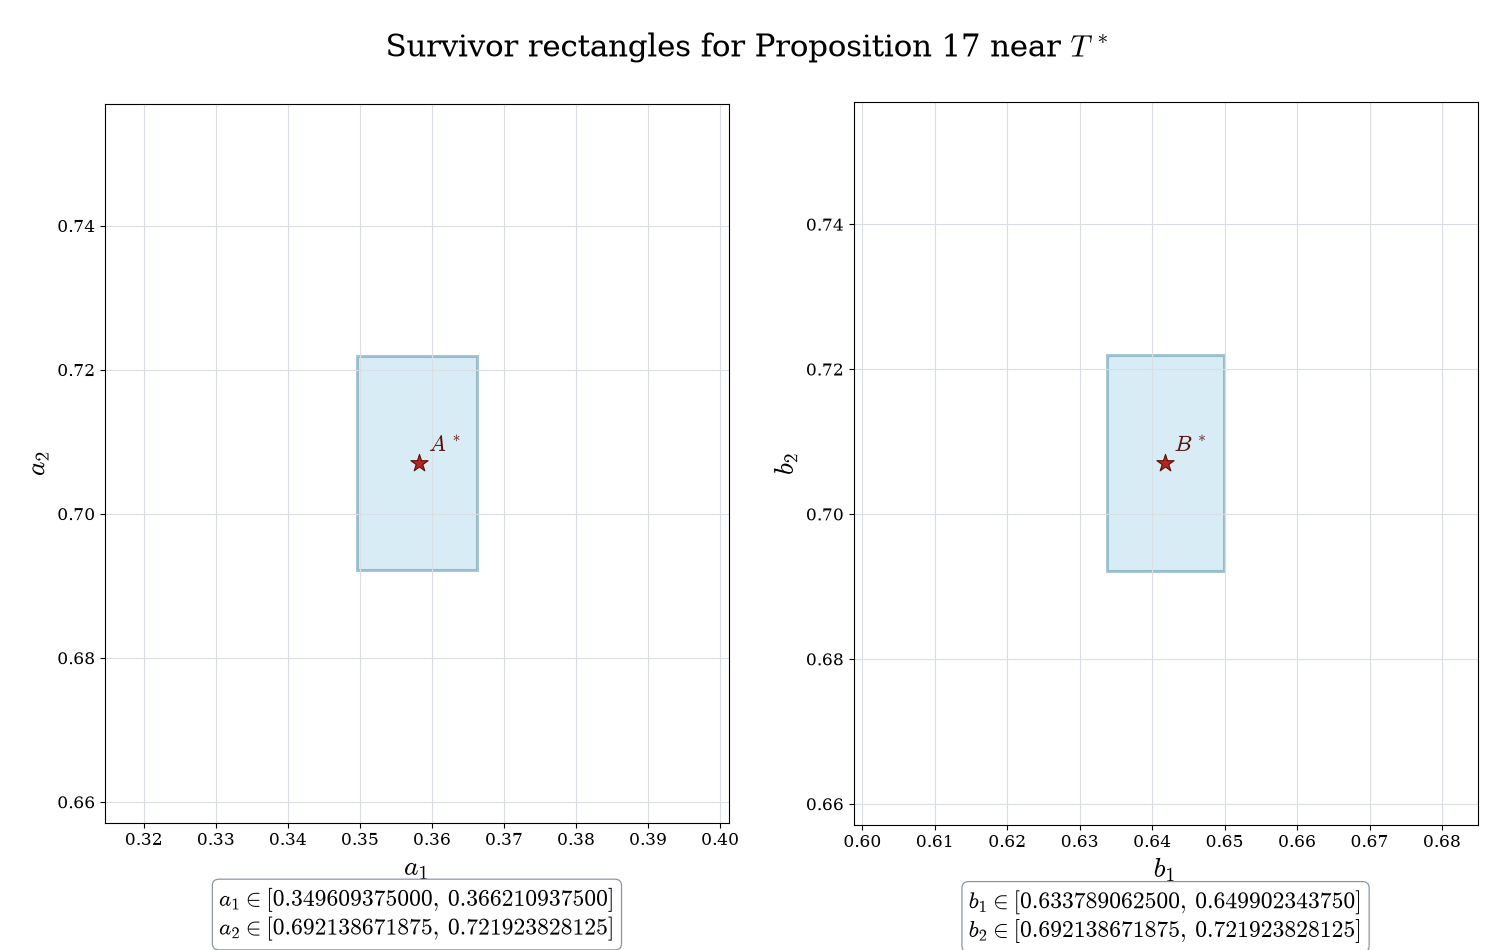
\includegraphics[width=0.86\textwidth]{figures/current_survivor_rectangles.png}
\caption{Equal-axis PNG export of the current survivor rectangles for \(A\) and
\(B\), together with the reference trapezoid point.  The left panel is the left
mobile vertex \(A\), and the right panel is the right mobile vertex \(B\).}
\end{figure}

\begin{figure}[h]
\centering
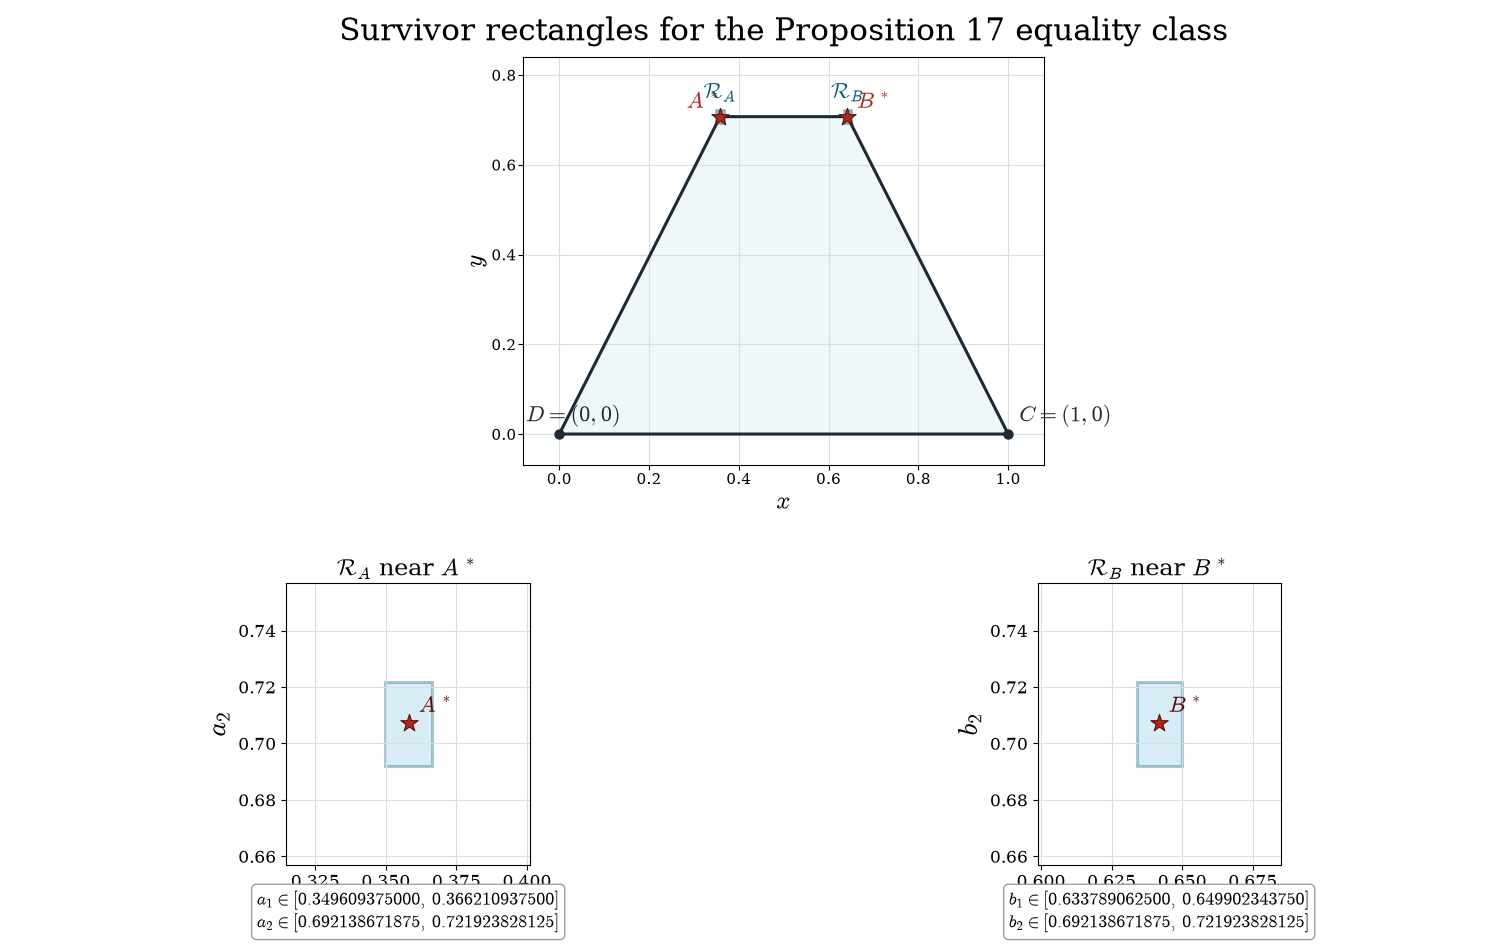
\includegraphics[width=0.92\textwidth]{figures/survivor_rectangles_overview.png}
\caption{Overview of the conjectured optimal trapezium \(DCB^\ast A^\ast\).
The survivor rectangles \(R_A\) and \(R_B\) are drawn in place and repeated as
zoomed sub-images inside the larger geometric view.}
\end{figure}

\subsection{Interpretation}

For threshold \(1.0496\), the recorded refinement sequence leaves only boxes inside
\(R_A\times R_B\).  Outside this product rectangle, every admissible normalized
quadrilateral is either certified to have shortest fence value at most
\(1.0496\) or proved incompatible with the opposite-pair equality hypothesis
of Proposition~17.  After the paper's analytic reduction to cases in which
both opposite-pair fences are active, there is therefore no possible
above-threshold candidate outside \(R_A\times R_B\).

This is stronger than the earlier run without auxiliary certificates, but it
must be read with the correct status semantics: \code{pair\_incompatible} is
not a low-fence estimate or a universal optimizer exclusion.  It is a separate
exclusion from the equality class.  Legacy certificates use the misleading
wire-format name \code{nonoptimal} for the same status.

\subsection{Audit Status}

The listed files are incremental refinement files: each refinement replaces the
survivor leaves of the preceding run.  Assemble the chain before whole-domain
verification:

\begin{lstlisting}
./fence_validate --assemble \
  flat_pair_cert_w0025.jsonl \
  flat_pair_refine_w00125.jsonl \
  flat_pair_refine_w000625.jsonl \
  flat_pair_refine_w0003125.jsonl \
  flat_pair_refine_w00015625.jsonl \
  flat_pair_refine_w000078125.jsonl \
  flat_pair_refine_w0000390625.jsonl \
  --out flat_pair_full_w0000390625.jsonl
\end{lstlisting}

The recorded assembly produced
\[
  799{,}546
\]
leaves.  The assembled full-domain certificate was then audited by

\begin{lstlisting}
./fence_validate --verify flat_pair_full_w0000390625.jsonl \
  --prec 70 --serial
\end{lstlisting}

with output
\[
\begin{aligned}
&799{,}546\text{ leaves},\quad 14{,}550\text{ discarded},\quad
500{,}767\text{ certified},\\
&213\text{ flat-area},\quad 265{,}491\text{ pair-incompatible},\quad
18{,}525\text{ survivors}.
\end{aligned}
\]
The dyadic partition coverage of the full root box passed, every Arb endpoint
comparison with the exact rational threshold passed, and the audit reported
zero failures.  The verifier printed
\(1.0495999994684\) as its rounded binary64 diagnostic for the largest
rechecked certified upper endpoint; the printed decimal is descriptive and is
not used for the proof comparison.

The historical assembled artifact has SHA-256
\begin{lstlisting}
58e3a555c83b54e90676062092eaa988da5bf247435949fa663a229921ad8000
\end{lstlisting}
Its recorded C source was unchanged since commit
\begin{lstlisting}
5bcd9694c66cbeab03515c624225f7398c74bc82
\end{lstlisting}
The final refinement was documented in commit
\begin{lstlisting}
c6dcd2dcebffad89d8143352f719bd6bfa83877b
\end{lstlisting}
This artifact predates the
present repair pass, but the repaired verifier has rechecked all 799,546 leaves
and the full dyadic cover successfully.  A publication package should archive
the compressed assembled JSONL beside a tagged repaired source revision and
publish its SHA-256 and the exact verifier commit.  Regeneration is optional;
it would canonicalize the legacy status spelling and requires its own hash and
source record.

Verifying a refinement-only file as a full certificate is now a fast structural
failure: the verifier reports the first missing dyadic child instead of
descending an empty subtree.

The verification command may additionally include \code{--theta 1.0496} and
\code{--form centered}; in the current code these are checked against the
metadata rather than used to define the certificate claim.

\section{Limitations and Soundness Notes}

\begin{itemize}
  \item Certification is based on upper bounds for the shortest fence.  A
  certified box proves ``below threshold'', while a survivor only means that
  the current candidate-value enclosures were not tight enough to certify.

  \item Status \code{pair\_incompatible} is not an upper-bound statement.  It
  certifies failure of the opposite-pair equality hypothesis in
  Proposition~17.  This is valid because the two pair intervals enclose exact
  pair-construction values for the sectors containing the quadrilateral.
  Conclusions using these leaves are conditional on the paper's active-pair
  analytic reduction.  Legacy JSONL status \code{nonoptimal} has the same
  limited meaning.

  \item Status \code{flat\_area} is an upper-bound statement.  It uses
  \(L_{DC,BA}/\sqrt {A_Q}\le 2\sqrt {A_Q}\) and \(A_{\rm ub}\le\theta^2/4\) to prove
  the box below threshold.

  \item Coarse boxes near degeneracies can have very wide interval enclosures.
  This is intentional: non-finite or loose enclosures force splitting or
  survival, never false certification.

  \item The JSONL enclosure printed in a certificate is diagnostic.  The
  verifier ignores the recorded enclosure and recomputes claims from the box,
  the metadata threshold, metadata form, metadata half-domain flag, and the
  requested verification precision.

  \item The metadata \code{theta} string is the exact proof threshold.  The
  \code{theta\_approx} field and printed threshold doubles are for human
  readability and adaptive search heuristics only.

  \item A run stopped by \code{--max-leaves} is useful for debugging but is not
  a complete certificate and should fail the full coverage check.

  \item Parallel execution uses a shared stack, so output order may vary.  The
  verifier sorts leaves and checks dyadic coverage, so certificate correctness
  does not depend on output order.
\end{itemize}

\end{document}
